\documentclass[a4paper,11pt,twoside,french]{article}
\usepackage[OT1]{fontenc} \usepackage[utf8]{inputenc}
\usepackage{babel}
\usepackage[a4paper,tmargin=2.5truecm,bmargin=3truecm,outer=2.5truecm,inner=2.5truecm,twoside,verbose=false %,showframe
]{geometry}

\usepackage{amsmath,amssymb,amsthm}
\usepackage{multicol}
\usepackage{enumitem}
\usepackage{graphicx}

\begin{document}

%    \begin{multicols}{2}

%\vfill\null
%\columnbreak
Amplitudes of the $f(t)$ functions, at selected center-of-mass energies, is shown on Figure \ref{ampl}. Greatest modulations of $t\bar{t}$ cross sections are expected in the benchmark scenarios $c_{XY} = c_{YX}$ and $c_{XX} = -c_{YY}$. The sensitivity is higher when probing components in the ecliptic plane.

At Tevatron, $t\bar{t}$ production was initiated mainly by $q\bar{q}$ annihilation while at the LHC, $gg$ fusion is dominant. We compare the $f(t)$ amplitude, between samples generated at the same center-of-mass energy $\sqrt{s} = 1.96$ TeV for D$\emptyset$ and CMS. We find similar amplitudes between D$\emptyset$ and CMS at $\sqrt{s} = 1.96$ TeV for the benchmarks $c_{XX} = -c_{YY} \neq 0$ and $c_{XY} = c_{YX} \neq 0$. However, at the same energy and production mechanism, the LHC position induces worst expected sensitivity to $c_{XZ} = c_{ZX} \neq 0$ and $c_{YZ} = c_{ZY} \neq 0$ benchmarks. We scanned the latitude and azimuth of poential experiments on earth and foiund that both ATLAS or CMS sit in a dip for the projected sensitivity on those SME coefficients.


%    \end{multicols}


    \begin{figure}[h!]
        \begin{center}
            \label{ampl}
            \includegraphics[scale=0.4]{amplEnergy_{XX}.eps}
            \includegraphics[scale=0.4]{amplEnergy_{XY}.eps}
            \includegraphics[scale=0.4]{amplEnergy_{XZ}.eps}
            \includegraphics[scale=0.4]{amplEnergy_{YZ}.eps}
            \caption{Amplitude for experiments D$\emptyset$, CMS (LHC), CMS (HL-LHC), CMS (HE-LHC) and FCC for all $c_{\mu \nu}$ benchmark}
        \end{center}
    \end{figure}

    \begin{figure}[h!]
        \begin{center}
            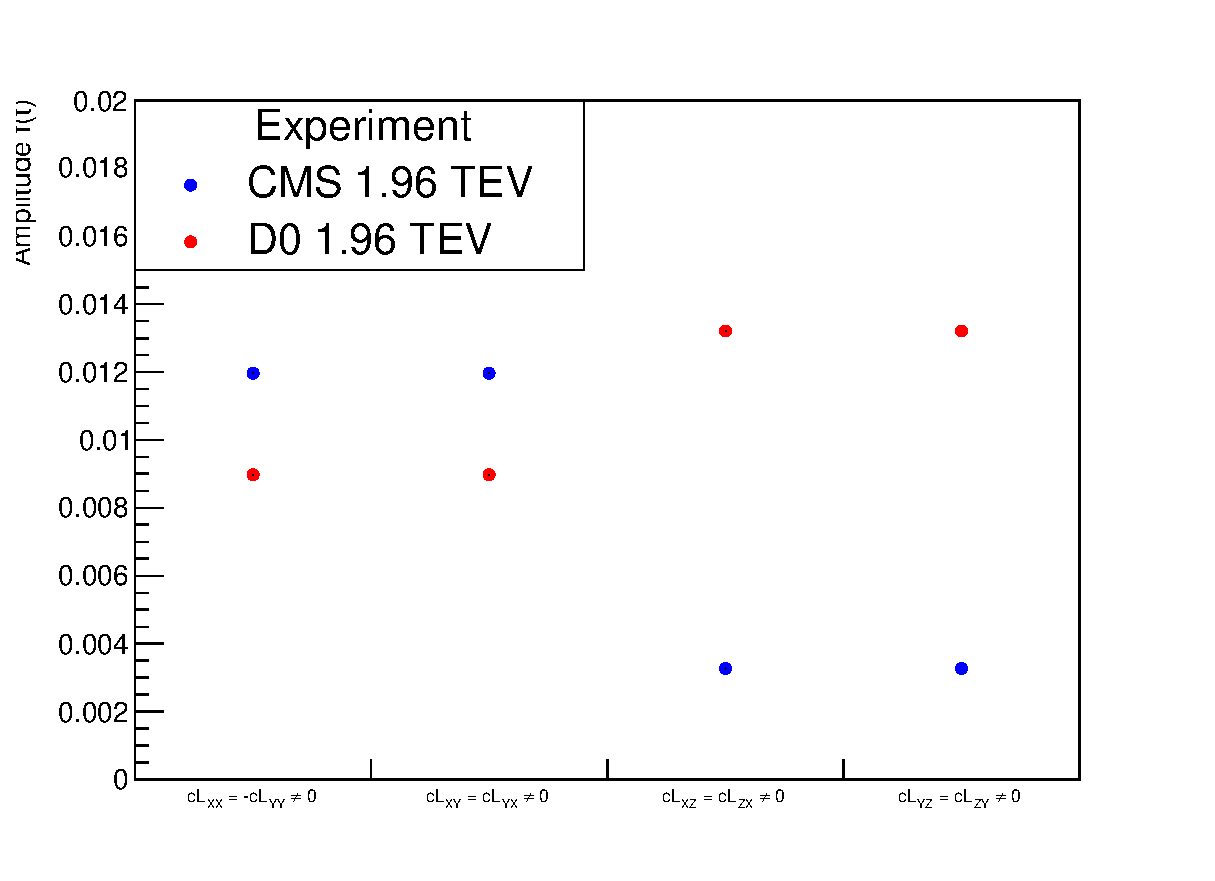
\includegraphics[scale=0.4]{compaCMSTEVL.eps}
            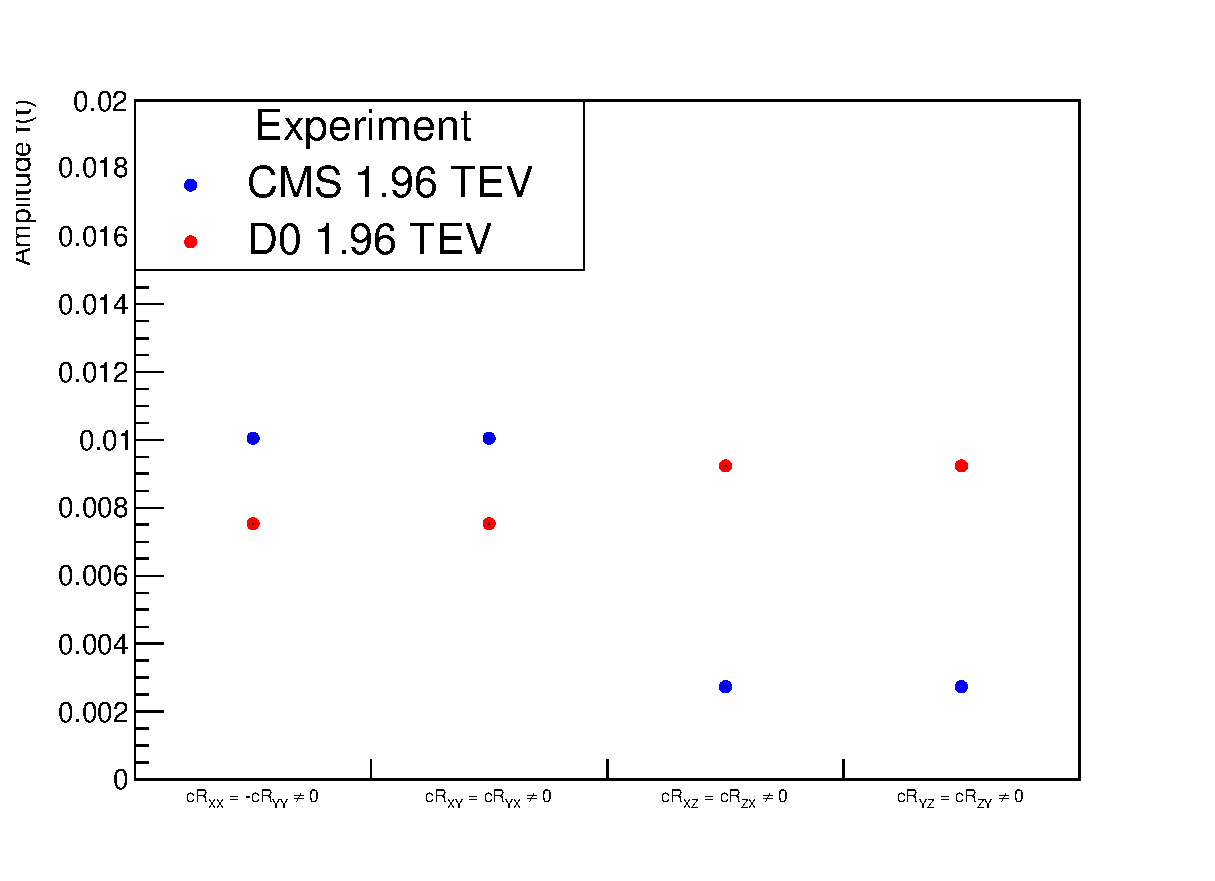
\includegraphics[scale=0.4]{compaCMSTEVR.eps}
            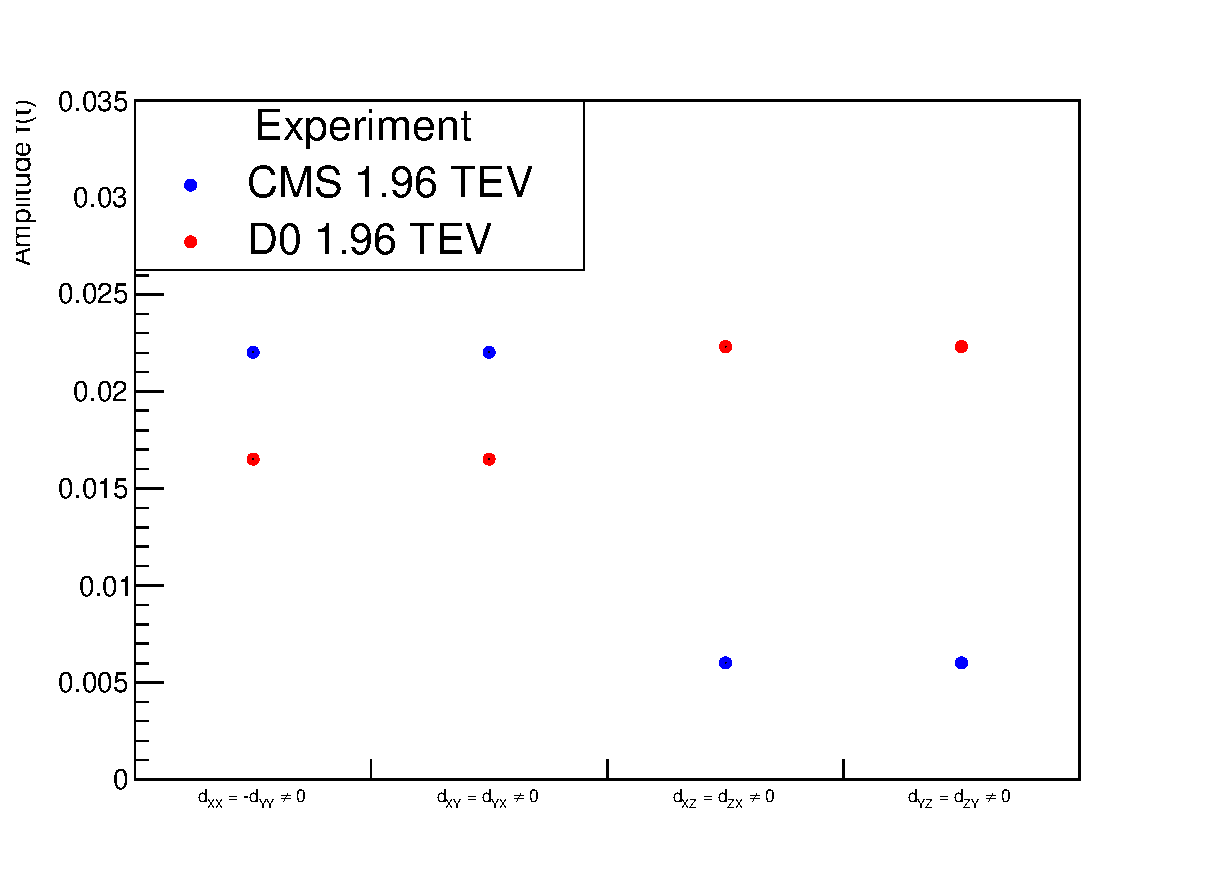
\includegraphics[scale=0.4]{compaCMSTEVD.eps}
            \caption{Amplitude comparaison for D$\emptyset$ and CMS at $\sqrt{s} = 1.96$ TeV}
        \end{center}
    \end{figure}

        \begin{multicols}{3}
            Experiment
        				\begin{itemize}[label=$\triangleright$]
            				\item Tev (D$\emptyset$)
            				\item LHC Run-II (CMS)
            				\item HL-LHC 
            				\item HE-LHC 
            				\item FCC 
        				\end{itemize}
            $c_{LXX} / c_{LXY}  $
        				\begin{itemize}[label=$\triangleright$]
            				\item $ \Delta c_{LXX} =1\times 10^{-1} $ 
            				\item $\Delta c_{LXX} =2\times 10^{-4} $
            				\item $\Delta c_{LXX} =2\times 10^{-5} $
            				\item $\Delta c_{LXX} =4\times 10^{-6} $
            				\item $\Delta c_{LXX} =1\times 10^{-6} $
        				\end{itemize}
            $c_{LXZ}  / c_{LYZ} $
   \begin{itemize}[label=$\triangleright$]
            				\item $\Delta c_{LXZ} =8\times 10^{-2} $
            				\item $\Delta c_{LXZ} =5\times 10^{-4} $
            				\item $\Delta c_{LXZ} =9\times 10^{-5} $
            				\item $\Delta c_{LXZ} =2\times 10^{-5} $
            				\item $\Delta c_{LXZ} =4\times 10^{-6} $
   \end{itemize}
        \end{multicols}

                        \begin{multicols}{3}
                            Expériences
            				\begin{itemize}[label=$\triangleright$]
                				\item Tev (D$\emptyset$)
                				\item LHC Run-II (CMS)
                				\item HL-LHC 
                				\item HE-LHC 
                				\item FCC 
            				\end{itemize}
                            $c_{RXX} / c_{RXY}  $
                			\begin{itemize}[label=$\triangleright$]
                				\item $\Delta c_{RXX} =9\times 10^{-2}$		
                				\item $\Delta c_{RXX} =4\times 10^{-4}$		
                				\item $\Delta c_{RXX} =9\times 10^{-5}$		
                				\item $\Delta c_{RXX} =2\times 10^{-5}$		
                				\item $\Delta c_{RXX} =5\times 10^{-6}$		
                			\end{itemize}
                            $c_{RXZ}  / c_{RYZ} $
                			\begin{itemize}[label=$\triangleright$]
                				\item $\Delta c_{RXZ} =7\times 10^{-2}$		
                				\item $\Delta c_{RXZ} =2\times 10^{-3}$		
                				\item $\Delta c_{RXZ} =3\times 10^{-4}$		
                				\item $\Delta c_{RXZ} =6\times 10^{-5}$		
                				\item $\Delta c_{RXZ} =2\times 10^{-5}$		
                			\end{itemize}
                        \end{multicols}

                        \begin{multicols}{3}
                            Expériences
            				\begin{itemize}[label=$\triangleright$]
                				\item Tev (D$\emptyset$)
                				\item LHC Run-II (CMS)
                				\item HL-LHC 
                				\item HE-LHC 
                				\item FCC 
            				\end{itemize}
                            $c_{XX} / c_{XY}  $
                			\begin{itemize}[label=$\triangleright$]
                				\item $\Delta c_{XX} =7\times 10^{-1}$		
                				\item $\Delta c_{XX} =2\times 10^{-4}$		
                				\item $\Delta c_{XX} =3\times 10^{-5}$		
                				\item $\Delta c_{XX} =6\times 10^{-6}$		
                				\item $\Delta c_{XX} =1\times 10^{-6}$		
                			\end{itemize}
                            $c_{XZ}  / c_{YZ} $
                			\begin{itemize}[label=$\triangleright$]
                				\item $\Delta c_{XZ} =6\times 10^{-1}$		
                				\item $\Delta c_{XZ} =6\times 10^{-4}$		
                				\item $\Delta c_{XZ} =1\times 10^{-4}$		
                				\item $\Delta c_{XZ} =2\times 10^{-5}$		
                				\item $\Delta c_{XZ} =4\times 10^{-6}$		
                			\end{itemize}
                        \end{multicols}

                        \begin{multicols}{3}
                            Expériences
            				\begin{itemize}[label=$\triangleright$]
                				\item Tev (D$\emptyset$)
                				\item LHC Run-II (CMS)
                				\item HL-LHC 
                				\item HE-LHC 
                				\item FCC 
            				\end{itemize}
                            $d_{XX} / d_{XY}  $
                			\begin{itemize}[label=$\triangleright$]
                				\item $\Delta d_{XX} = 9.9\times 10^{-2}$
                				\item $\Delta d_{XX} = 9.5\times 10^{-5}$
                				\item $\Delta d_{XX} = 1.8\times 10^{-5}$
                				\item $\Delta d_{XX} = 3.4\times 10^{-6}$
                				\item $\Delta d_{XX} = 7.8\times 10^{-7}$
                			\end{itemize}
                            $d_{XZ}  / d_{YZ} $
                			\begin{itemize}[label=$\triangleright$]
                				\item $\Delta d_{XZ} = 7.2\times 10^{-2}$		
                				\item $\Delta d_{XZ} = 3.5\times 10^{-4}$		
                				\item $\Delta d_{XZ} = 6.8\times 10^{-5}$		
                				\item $\Delta d_{XZ} = 1.2\times 10^{-5}$		
                				\item $\Delta d_{XZ} = 2.9\times 10^{-6}$		
                			\end{itemize}
                        \end{multicols}

\end{document}